% Intended LaTeX compiler: pdflatex
\documentclass[10pt,a4paper,UTF8]{article}
\usepackage{zclorg}
\usepackage{tikztheorem}
\author{zcl.space}
\date{}
\title{信道编码理论中用到的代数基础}
\hypersetup{
 pdfauthor={zcl.space},
 pdftitle={信道编码理论中用到的代数基础},
 pdfkeywords={communication algebra math},
 pdfsubject={本文总结差错控制编码第二章。},
 pdfcreator={Emacs 25.2.1 (Org mode 9.0.9)},
 pdflang={English}}
\begin{document}

\maketitle
\tableofcontents
\titlepic{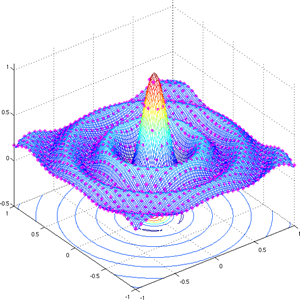
\includegraphics[scale=0.25]{../../img/sinc.PNG}}
本章的内容是信道编码理论中用到的最基本的抽象代数的汇总。林舒也无意让读者通过本章的学习掌握抽象代数。更详细的抽象学习推荐其他教材,当然在本章结尾本书作者也推荐了一些经典老教材。此处,我推荐Michael Artin的《代数》和Harvard大学与此书配套的公开课。

当然本章也并不是没有存在必要。本章以较快的节奏给出了信道编码理论中涉及的代数理论,便于有一定基础的专业人士快速复习和进入编码世界。

\section{群}
\label{sec:org72e8b21}


群是抽象代数中最基本的概念。假设 \(G\)是一个集合,在\(G\)上,我们定义一个二元运算规则 \(*\)。通过这个二元运算规则和 \(G\)中的任意两个元素 \(a\)和\(b\),我们可以定义第三个元素 \(c=a*b\). 当\(c\in G\),我们称 \(*\)在 \(G\)上是封闭的。比如,假设\(G\)是所有整数的集合,二元运算是加法,则对于 \(G\)中的任意整数 \(i\)和\(j\),有\((i+j)\in G\)。我们称所有整数组成的集合在加法下是封闭的。 二元运算 \(*\)满足结合律,当且仅当 \(\forall a,b,c\in G\):\[a*(b*c) = (a*b)*c\] 现在我们给出群的完整定义:

在一个集合\(G\)上定义二元运算,当满足以下条件时我们称\(G\)是一个群:
\begin{enumerate}
\item 二元运算满足结合律;
\item \(G\)中有一个元素 \(e\), \(\forall a\in G\)满足: \[a*e = e*a = a\]我们称\(e\)是单位元素。
\item \(\forall a\in G\), \(G\)中有一个元素\(a^{'}\) 满足: \[a*a^{'} = a^{'}*a = e\] 我们称\(a^{'}\)是逆元。
\end{enumerate}

群\(G\)是交换群,当且仅当对于任何两个元素 \(a,b\in G\),有 \[a*b=b*a\] 对于群\(G\),单位元素\(e\)和逆元都是唯一存在的。对于整数加法群,单位元是\(0\),\(-i\)是\(i\)的逆元。所有除0以外的有理数构成一个乘法交换群:单位元是\(1\),\(b/a\)是\(a/b\)的逆元。无论是整数加法群还是除零外的有理数乘法群,其元素个数都是无穷多个。当然,只有有限个元素的群也是存在的,我们称这样的群为有限群。

接下来考虑一个集合 \(G = \{0,1\}\),这个集合只有两个元素,并定义一个二元运算:\[0\oplus 0 =0, 0\oplus 1=1, 1\oplus 0 = 1, 1\oplus 1 = 0\] 我们称这样的二元运算为模二加。显然,定义了\(\oplus\)运算的集合\(G\)是一个交换群。

群中元素的个数叫做群的阶数。具有有限阶的群叫做有限群。接下来我们来阐述一个事实:对于任何的正整数\(m\),我们都有可能定义一个有限群,群上的二元运算与实数加法非常相似。考虑一个整数集合\(G=\{0,1,2,\ldots,m-1\}\)  定义\(+\)是实数加法,定义\(\boxplus\)是\(G\)上的二元运算满足 \[i\boxplus j = r \] 其中 \(r = i+j \mod(m)\), 我们称其为模\(m\)加。显然\(0 \leq r \leq (m-1)\) 并且\(r\in G\).因此在二元运算符号\(\boxplus\)运算下 \(G\)是封闭的。对于 \(0 < i < m\) , \(i\)和\(m-i\)都在\(G\)中. 因为 \[i + (m-i) = (m-i) + i = m\] 所以有\[i\boxplus (m-i) = (m-i)\boxplus i = 0\] 因此,\(i\)和\(m-i\)在\(\boxplus\)运算下互逆。\(0\)的逆是它本身。另外我们还可以证明模\(m\)加满足结合律,即\[(i\boxplus j)\boxplus k = i \boxplus ( j \boxplus k)\] 综上,我们可以说集合\(G=\{0,1,2,\ldots,m-1\}\)在模\(m\)加运算下是一个群。我们称这样的群为加法群。我们给出一个模4加群计算中的模4加表如下所示:

\begin{table}[htbp]
\caption{\label{tab:org2011b09}
模4加法表}
\centering
\begin{tabular}{rrrrr}
\hline
\(\boxplus\) & 0 & 1 & 2 & 3\\
\hline
0 & 0 & 1 & 2 & 3\\
1 & 1 & 2 & 3 & 0\\
2 & 2 & 3 & 0 & 1\\
3 & 3 & 0 & 1 & 2\\
\hline
\end{tabular}
\end{table}

接下来我们看一个乘法交换群的例子。假设\(p\)是一个素数,考虑集合\(G = \{1,2,3,\ldots,p-1\}\)。我们定义\(\cdot\)为乘法,定义\(\boxdot\) 为模p乘,具体表示为 \[i\boxdot j = r, r = i\cdot j \mod p\] 首先我们知道\(i\cdot j\)不能被\(p\)整除,因此 \(0 < r < p\) 且\(r\)是\(G\)中的一个元素。进而得出,\(r\)是\(G\)中的一个元素。可以证明在模p乘运算下,\(G\)是一个交换群。

显然\(1\)是单位元素。接下来我们证明对于每一个元素\(i\)都有且只有一个逆元存在。由于\(p\)是一个素数,\(i < p\), \(i\)和\(p\)之间没有任何大于1的公约数。另外根据欧几里德定理存在两个整数满足 \[a\cdot i + b\cdot p = 1\] 其中\(a,p\)之间没有除1之外的最大公约数。把上式重排,我们有 \[a\cdot i = -b\cdot p +1\] 这说明\(a\)是 \(i\)在\(G\)中模\(p\)乘的逆。值得一提的是当\(p\)不是质数时,\(G\)不是群。

接下来我们定义子群的概念。假定\(H\)是群\(G\)的一个子集,那么\(H\)是群\(G\)的一个子群当且仅当\(H\)在群\(G\)中的运算下是封闭的。

\emph{定理} 假设\(G\)是二元运算\(*\)下的群。\(H\)是\(G\)的一个子集,那么\(H\)是一个子群,当且仅当:
\begin{enumerate}
\item \(H\)在二元运算\(*\) 下封闭;
\item 对于\(H\)中的任何一个元素\(a\),其逆也在\(H\)中。
\end{enumerate}

接下来我们顶一个非常重要的概念:陪集。假设\(H\)是\(G\)的一个子群,二元运算为\(*\),假设\(a\)是\(G\)中的任何一个元素。那么集合 \(a*H \triangleq \{a*h: h\in H\}\)叫做 \(H\)的左陪集;集合 \(H*a \triangleq \{h*a: h\in H\}\)叫做 \(H\)的右陪集。显然,当\(G\)是交换群的时候,左陪集等于右陪集。

考虑一个模16加法群\(G = \{0,1,2,\ldots,15\}\)。可以检验\(H= \{0,4,8,12\}\)是一个子群。对于这个子群有陪集:
\begin{eqnarray*}
0\boxplus H &=& \{0,4,8,12\} \\
1\boxplus H &=& \{1,5,9,13\} \\
2\boxplus H &=& \{2,6,10,14\} \\
3\boxplus H &=& \{3,7,11,15\}
\end{eqnarray*}
事实上,我们可以检验对于\(H\)只有这\(4\)个陪集。这\(4\)个陪集是互斥的,他们的并集构成了\(G\).

\emph{定理} 子群\(H\)的任意两个陪集的交集是空集。

假设\(a*H\)和\(b*H\)是\(H\)的两个不同的陪集,且\(a*h\)和\(b*h^{'}\)是\(a*H\)和\(b*H\)中的两个元素。假设\(a*h = b*h^{'}\),\(h^{-1}\)是\(h\)的逆。则有:
\begin{eqnarray*}
(a*h)*h^{-1}&=&(b*h^{'})*h^{-1} \\
a*(h*h^{-1})&=&b*(h^{'}*h^{-1}) \\
a*e &=& b* h^{''} \\
a &=& b*h^{''}
\end{eqnarray*}
其中 \(h^{''} = h^{'}*h^{-1}\) 是\(H\)中的一个元素。 \(a=b*h^{''}\)意味着:
\begin{eqnarray*}
a*H&=& (b*h^{'})*H \\
&=&\{(b*h^{''})*h:h\in H\} \\
&=&\{b*(h^{''}*h):h\in H\} \\
&=&\{b*h^{''''},h^{'''}\in H\}
&=& b*H
\end{eqnarray*}
此时,\(a*H\)和\(b*H\)是两个相同的陪集,与假设矛盾。

通过以上几个定理,我们发现群\(G\)的子集\(H\)的陪集具有以下性质:
\begin{enumerate}
\item 每一个\(G\)中的元素只出现在\(H\)的一个陪集中。
\item \(H\)的所有陪集是互斥的,即没有相同的元素。
\item \(H\)的所有陪集构成群\(G\),即\(H\)的所有陪集是群\(G\)的一个划分我们用\(G/H\)来表示。
\end{enumerate}

\emph{定理} (\textbf{朗格朗日定理}) 假设\(G\)是一个阶数为\(n\)的群,\(H\)是其阶数为\(m\)的子群。那么\(m\)可以整除\(n\),并且\(G/H\)有\(n/m\)个\(H\)的陪集。

\section{域}
\label{sec:org1cfe7b5}


现在基于群的概念,我们引入抽象代数的另一个概念:域。粗略来讲,域是一些元素的集合,在这个集合中加减乘除都是封闭的。并且加法,乘法满足交换律,结合律和分配率。域的正式定义如下:

\emph{定义} (\textbf{域}) 令\(F\)是一个集合,在该集合上定义两个双目运算:加法\(+\)和乘法\(\cdot\). 定义了加法和乘法运算的集合\(F\)是一个域,当且仅当:
\begin{enumerate}
\item \(F\)是一个加法交换群。零元是\(0\);
\item \(F\)中除\(0\)以外的元素是一个乘法交换群。乘法单位元用\(1\)表示。
\item \(F\)乘法满足分配率,即对\(F\)中的三个元素 \(a,b,c\)满足 \(a\cdot ( b+c) = a\cdot b + a\cdot c\)
\end{enumerate}

通过以上定义,我们知道域中必须包含两个元素:加法零元和乘法单位元。域的元素个数叫做域的阶数。如果一个域中元素个数是有限的,我们称这个域是有限域。在一个域中,定义元素\(a\)的加法逆元为\(-a\);乘法逆元为\(a^{-1},a\neq 0\)。从一个域元\(a\)中减去另一个元素\(b\)定义为\(a\)加上\(b\)的逆元 \(-b\)。如果\(b\)是一个非零元,则定义\(a\)除以\(b\)为\(a\)乘以\(b\)的逆元\(b^{-1}\)。

从域的定义中可以推导出域的一些基本性质:
\begin{enumerate}
\item 对于域中每一个元素\(a\), \(a\cdot 0 = 0\cdot a = 0\)
\item 对于域中任何两个非零元素\(a\)和\(b\),有\(a\cdot b \neq 0\)
\item \(a\cdot b = 0 a\neq 0\)意味着:\(b\neq 0\)
\item 对于域中任何两个元素 \(a\)和\(b\),有\(-(a\cdot b) = (-a)\cdot b = a\cdot (-b)\)
\item 对于\(a\neq 0,a\cdot b = a\cdot c\),有\(b = c\)
\end{enumerate}

易得,实数在实数加法和乘法下是一个域。这个域有无穷多个元素。接下来我们给一个有限域的例子。

考虑带有模2加法和乘法的集合\(\{0,1\}\)
\begin{table}[htbp]
\caption{\label{tab:orgfc1db57}
模2加法表}
\centering
\begin{tabular}{rrr}
+ & 0 & 1\\
\hline
0 & 0 & 1\\
1 & 1 & 0\\
\end{tabular}
\end{table}

\begin{table}[htbp]
\caption{\label{tab:orge53012e}
模2乘法表}
\centering
\begin{tabular}{rrr}
\(\cdot\) & 0 & 1\\
\hline
0 & 0 & 0\\
1 & 0 & 1\\
\end{tabular}
\end{table}

我们知道\(\{0,1\}\)是一个模2加交换群,\(\{1\}\)是一个模2乘群。同样我们可以很容易的验证模2乘在模2乘下满足分配率。

上面例子中的群我们成为二进制域,用\(GF(2)\)表示。\(GF(2)\)是一个非常重要的二进制域,这个域在编码理论,计算机理论和通信与存储系统中有广泛的应用。

接下来我们再给一个质数域的例子。假设\(p\)是一个素数了,那么\(\{0,1,2,\ldots,p-1\}\)是一个模\(p\)加下的交换群,同样我们也知道\(\{1,2,\ldots,p-1\}\)形成了模\(p\)的乘法交换群。根据模\(p\)加法和乘法定义,结合实数乘法在模\(p\)加法下满足乘法分配率。所以,\(\{0,1,2,\ldots,p-1\}\)是一个\(p\)阶域。由于这个域是从质数构造而来的所以这个域也叫作质数域。特别的当\(p=2\)时,我们有\(GF(2)\)。

以\(p=7\)为例,集合\(0,1,2,3,4,5,6\)是一个模\(7\)加法和乘法下的\(7\)阶域,用\(GF(7)\)表示。加法表对减法也适用。比如,如果我们要计算\(3-6\),首先我们找到\(-6\)的加法逆\(1\)。然后,把\(1\)和\(3\)相加,既得\(4\)。对于除法,我们使用乘法表。假设要计算\(\frac{3}{2}\),则我们首先找到\(2^{-1}\)的逆\(3\cdot 4 = 5\)。综上,我们验证了在一个有限域中,加法减法乘法除法可以像普通的代数运算一样进行计算。

我们知道对于任何的质数\(p\),存在一个\(p\)阶的有限域。事实上,对于任何的正整数\(m\),可以扩展质数域\(GF(p)\)到\(p^{m}\)个元素。更进一步,已经证明任何有限域的阶数是质数的幂次方。有限域也叫伽罗华域,这是为了纪念有限域的发明者:法国数学家伽罗华。很大一部分的代数编码理论,码的构建和译码都是基于有限域展开的。在接下来的几个章节,我们会考察有限域的几个基本性质:包括他们的代数结构,质数扩展域的构造。

考虑一个\(q\)阶有限域,\(GF(q)\),让我们做以下加法:
\begin{eqnarray*}
\sum_{i=1}^{1}1 &=& 1 \\
\sum_{i=1}^{2}1 &=& 1+1 \\
\sum_{i=1}^{3}1 &=& 1+1+1 \\
\ldots &=& \ldots \\
\sum_{i=1}^{k}1 &=& \underbrace{1+1+\ldots+1}_{k}
\end{eqnarray*}
因为有限域在加法下是封闭的,这些和一定在有限域中;又由于有限域中的元素个数是有限的,这些和不可能无限的加下去而不出现重复。因此在些和组成的序列中一定存在重复,即一定存在两个正整数\(m\)和\(n, m < n\) 且满足\[\sum_{i=1}^{m}1=\sum_{i=1}^{n} 1\] 这意味着\(\sum_{i=1}^{n-m}1=0\)。因此一定存在一个最小的正整数\(\lambda\)满足\(\sum_{i=1}^{\lambda}1=0\),我们称\(\lambda\)为\(GF(q)\)的特征值。二进制域\(GF(2)\)的特征值是2,因为\(1+1=0\)。更进一步,质数域\(GF(p)\)的特征值是\(p\)。因为\(\sum_{i=1}^{k}1 = k \neq 0, \forall 1\leq k < p\) 并且 \(\sum_{i=1}^{p}1 = 0\)

\emph{定理} 有限域的特征值\(\lambda\)是一个质数。
假设\(\lambda\)不是一个质数,那么\(\lambda\)可以表示成两个整数的乘积\(\lambda = km\),由于域在乘法下是封闭的,则有\[\left(\sum_{i=1}^{k}1  \right)\cdot \left(\sum_{i}^{m}1\right) \]也是域中的一个元素 利用分配率,有\[\left(\sum_{i=1}^{k}1  \right)\cdot \left(\sum_{i}^{m}1\right) = \sum_{i}^{km}1\] 由于\(\sum_{i}^{km}1 = 0\) 则,\(\sum_{i}^{k}1\)或者\(\sum_{i}^{m}1\)中至少有一个为0;然而这是不可能的,因为\(\lambda\)是满足\(\sum_{i}^{\lambda}1 = 0\)的最小整数。矛盾产生,因此\(\lambda\)是一个质数。

因此,我们可以进一步推论,对于\(GF(p)\)中的任何两个小鱼\(\lambda\)的正整数\(k,m\),有\[\sum_{i}^{k}1 \neq \sum_{i}^{k}1 \neq 0\] 同样我们可以用反证法来证明,假设\[\sum_{i}^{k}1 \neq \sum_{i}^{k}1\] 则有\[\sum_{i}^{k-m}1  = 0\], 不失一般性我们假设\(k > m\). 然而这是不可能的,因为\(k - m < \lambda\)

接下来我们有\(\lambda\)个不相同的数:\[1= \sum_{i}^{1}1, \sum_{i}^{2}1,\sum_{i}^{3}1, \ldots, \sum_{i}^{\lambda -1}1, \sum_{i}^{\lambda}1=0\]. 事实上,这个求和集合本上构成了加法和乘法下阶数为\(\lambda\)的域。由于\(GF(\lambda)\)是\(GF(q)\)的一个子集,我们称\(GF(\lambda)\)是\(GF(q)\)的一个子域. 因此,我们可以说任何特征为\(\lambda\) 的域\(GF{q}\)都有子域\(GF(\lambda)\). 另外可以证明 \textbf{如果\(\lambda \neq q\),那么\(q\)是\(\lambda\)的幂次方}

现在,假设\(a\)是域\(GF(q)\)中的一个非零元素。由于\(GF(q)\)中的所有非零元素在乘法下是封闭的,则下面的\(a\)的幂次方序列\[a^{1} = 1, a^{2}= a\cdot a, a^{3}=a\cdot a \cdot a,\ldots\] 一定全都是\(GF(q)\)中的非零元素。又因为\(GF(q)\)中元素的格式是有限的,所以\(a\)的幂次方序列中元素个数肯定不可能是无限的。因此,在某个点上,一定会出现重复,即:一定有两个整数\(k,m, m > k\),且\(a^{m} = a^{k}\)。定义\(a^{-1}\)是\(a\)的逆。则有\((a^{-1})^{k} = a^{-k}\)是\(a^{k}\)的逆。在\(a^{m} = a^{k}\)两边乘\(a^{k}\)的逆,则有\(a^{m-k} = 1\)。这个等式说明一定存在一个最小的正整数\(n\)满足\(a^{n}=1\),我们称这个整数是元素\(a\)的阶。因此序列\(a,a^{2},a^{3},\ldots\)在\(a^{n}=1\)之后重复。同时,\(a^{1},a^{2},a^{3},\ldots,a^{n-1},a^{n}=1\)互不重复。事实上,这个序列中的元素集合构成了\(GF(q)\)下的乘法群。首先,我们知道这个集合包含单位元\(1\),然后考虑\(a^{i}\cdot a^{j}\),如果\(i+j\leq n\) 则\(a^{i}\cdot a^{j} = a^{i+j}\)。如果\(i+j > n\),我们有\(i+j = n +r, 0 < r \leq n\),因此\[a^{i}\cdot a^{j} = a^{i+j} = a^{n}\cdot a^{r} = a^{r}\] 因此,幂序列\(a^{1},a^{2},a^{3},\ldots,a^{n-1},a^{n}=1\) 在\(GF(q)\)乘法下是封闭的。\(a^{n-i}, 1\leq i < n\)的逆是\(a^{i}\)。又因为\(a\)的幂在\(GF(q)\)中是非零的,它们又满足交换路和结合律。因此\(a^{1},a^{2},a^{3},\ldots,a^{n-1},a^{n}=1\)构成了\(GF(q)\)下的交换群。

如果群中的一个元素的幂构成这个群中的所有元素,那么这个群是交换群。

\emph{定理} 如果\(a\)是有限域\(GF(q)\)中的非零元素,那么\(a^{q-1}=1\)

证明:假设\(b_{1},b_{2},\ldots,b_{q-1}\)是\(q-1\)个\(GF(q)\)的非零元素,那么\(q-1\)个元素\(a\cdot b_{1}, a\cdot b_{2}, \ldots , a\cdot b_{q-1}\)非零且各不相同。因此:
\begin{eqnarray*}
(a\cdot b_{1})\cdot (a\cdot b_{2}) \cdot (a\cdot b_{q-1})&=&b_{1}\cdot b_{2}\ldots b_{q-1} \\
a^{q-1}\cdot (b_{1}\cdot b_{2}\ldots b_{q-1}) &=& b_{1}\cdot b_{2}\ldots b_{q-1}
\end{eqnarray*}
由于\(a\neq 0\) 并且\(b_{1}\cdot b_{2}\ldots b_{q-1}\neq 0\),因此\(a^{q-1}=1\)

\emph{定理} 令\(a\) 是\(GF(q)\)域的非零元素,\(n\)是\(a\)的阶数,则\(n\)整除\(q-1\)

证明:采用反证法。假设\(n\)不整除\(q-1\),则\[q-1 = kn +r, 0 < r < n \] \[a^{q-1} = a^{kn+r} = a^{kn}a^{r}\]
因为\(a^{q-1} = a^{n} =1\)所以一定有\(a^{r}=1\) 因为 \(0 < r < n\)且\(n\)是满足\(a^{n}=1\)的最小整数 ,矛盾产生。因此 \(n\)一定整除\(q-1\).

在有限域\(GF(q)\)中 ,一个非零元素\(a\)是本源的,如果\(a\)的阶数是\(q-1\). 因此一个域的本源元素生成了该域中的所有非零元素。每一个有限域中含有一个本源元素。

以\(GF(7)\)为例,该域的特征值为\(7\), 如果我们计算\(3\)的幂会
\begin{eqnarray*}
3^{1}&=&3 \\
3^{2}&=&2 \\
3^{3}&=&6 \\
3^{4}&=&4 \\
3^{5}&=&5 \\
3^{6}&=&1
\end{eqnarray*}
我们发现\(3\)的阶数是\(6\),并且\(3\)生成了所有的\(GF(7)\)中的元素,所以\(3\)是\(GF(7)\)中的本源元。对于整数\(4\),我们有
\begin{eqnarray*}
4^{1}&=&4 \\
4^{2}&=&2 \\
4^{3}&=&1
\end{eqnarray*}
因此\(4\)的阶数是\(3\),\(3\)是\(6\)的一个因子。
\section{二进制域代数}
\label{sec:org935f612}


原则上讲,基于\(GF(q)\) (\(q\)是质数或者质数的幂),我们可以构建任何编码方案。但是在数字通信系统中,基于\(GF(2)\)或者\(GF(2^{m})\)的码是用的最多的编码方案。因此在这一节我们着重讨论二进制域上的代数运算。

在二进制域中,我们使用模\(2\)的加法和乘法。事实上这些代数和普通的代数运算没有什么区别,需要注意的是在\(GF(2)\)中\(2=0\).比如\(1+1=2=0\)。另外需要注意\(1+1=0\)所以\(1=-1\)。因此在二进制域中减法等于加法。为了演示在二进制域中的计算我们考虑下面的方程组:
\begin{eqnarray*}
X+Y&=&1 \\
X+Z&=&0 \\
X+Y+Z&=&1 \\
\end{eqnarray*}
这个方程可以通过第一和第三个方程相加,得到\(Z=0\)。然后,利用第二个方程,得\(X=0\);利用第一个方程\(Y=1\)。

因为我们可以唯一解这个方程,所以这个方程一定是线性独立的,左边部分行列式的值一定非零。如果行列式值非零又是在\(GF(2)\)上的行列式,那么行列式一定\(1\)。因此我们可以通过Cramer准则解这个方程。
\begin{equation*}
\label{eq:1}
X=
\frac{
\begin{vmatrix}
1& 1& 0 \\
0& 0& 1 \\
1& 1& 1
\end{vmatrix}
}{
\begin{vmatrix}
1& 1& 0 \\
1& 0& 1 \\
1& 1& 1
\end{vmatrix}
}
= \frac{0}{1} = 0
\end{equation*}
\begin{equation*}
Y=
\frac{
\begin{vmatrix}
1& 1& 0 \\
1& 0& 1 \\
1& 1& 1
\end{vmatrix}
}{
\begin{vmatrix}
1& 1& 0 \\
1& 0& 1 \\
1& 1& 1
\end{vmatrix}
}
= \frac{1}{1} = 1
\end{equation*}
\begin{equation*}
Z=
\frac{
\begin{vmatrix}
1& 1& 1 \\
1& 0& 0 \\
1& 1& 1
\end{vmatrix}
}{
\begin{vmatrix}
1& 1& 0 \\
1& 0& 1 \\
1& 1& 1
\end{vmatrix}
}
= \frac{0}{1} = 0
\end{equation*}
接下来我们考虑计算\(GF(2)\)域的多项式计算。单变量多项式\(f(X)\)表示为:
\begin{equation}
\label{eq:3}
f(X) = f_{0} + f_{1}X + f_{2}X^{2} + \ldots + f_{n}X^{n}
\end{equation}
其中\(f_{i}=0\)或者\(1\)。多项式的度是多项式中具有非零洗漱的\(X\)的最大幂次。如果\(f_{n}=1\),那么\(f(X)\)是一个度为\(n\)的多项式。如果\(f_{n}=0\),那么\(f(X)\)是一个度小于\(n\)的多项式。\(f(x) = f_{0}\)的度是\(0\)。

一共有两个度为\(1\)的多项式,分别是\(X\)和\(1+X\)。一共有四个度为\(2\)的多项式:非别是\(X^{2},1+X^{2},X+X^{2},1+X+X^{2}\). 推而广之,一共有\(2^{n}\)个度为\(n\)的\(GF(2)\)多项式。

\(GF(2)\)多项式可以执行加减乘除运算。假设\[g(x) = g_{0} + g_{1}X + g_{2}X^{2} + \ldots + g_{m}X^{m}\],则
\begin{equation*}
\label{eq:4}
f(X) + g(X) = (f_{0} + g_{0}) + (f_{1} + g_{1})X + \ldots + (f_{m} + g_{m})X^{m} + f_{m+1}X^{m+1} + \ldots + f_{n}X^{n}
\end{equation*}
其中\(f_{i} + g_{i}\)是模\(2\)加。例如,\(a(X) = 1+ X + X^{3} + X^{5}\) \(b(X) = 1 + X^{2} + X^{3} + X^{4} + X^{7}\)。我们有:
\begin{eqnarray*}
a(X) + b(X) &=& (1+1) +  X + X^{2} + (1+1)X^{3} + X^{4} + X^{5} + X^{7} \\
            &=& X + X^{2} + X^{4} + X^{5} + X^{7}
\end{eqnarray*}
当我们\(f(X)\)和\(g(X)\)相乘时,有:
\[f(X)\cdot g(x) = c_{0} + c_{1}X + c_{2}X^{2} + \ldots + c_{n+m}X^{n+m}\]
其中:
\begin{eqnarray*}
c_{0}&=&f_{0}g_{0} \\
c_{1}&=&f_{0}g_{1} + f_{1}g_{0} \\
c_{2}&=&f_{0}g_{2} + f_{1}g_{1} + f_{2}g_{0} \\
\vdots &=& \vdots \\
c_{i}&=&f_{0}g_{i} + f_{1}g_{i-1} + f_{2}g_{i-1} + \ldots + f_{i}g_{0} \\
\vdots &=& \vdots \\
c_{n+m} &=&f_{n}g_{m}
\end{eqnarray*}
乘法和加法结果中的系数都是\(GF(2)\)中计算得出的。显然如果\(g(X)=0\)则\(f(X)\cdot 0 =0\). 我们可以很快确认在二进制域中,多项式满足如下性质:

\textbf{交换律}  :
\begin{eqnarray*}
a(X) + b(X)&=& b(X) + a(X) \\
a(X)\cdot b(X)&=&b(X)\cdot a(X)
\end{eqnarray*}
\textbf{结合律} :
\begin{eqnarray*}
a(X) + [b(X) + c(X)]&=& [a(X)+b(X)] + c(X) \\
a(X)\cdot [b(X)\cdot c(X)] &=&[a(X)\cdot b(X)]\cdot c(X)
\end{eqnarray*}
\textbf{分配率} :
\begin{equation*}
a(X)\cdot [b(X) + c(X)] = a(X)\cdot b(X) + a(X)\cdot c(X)
\end{equation*}

假设\(g(X)\)是非零多项式,则用\(g(X)\)去除\(f(X)\)我们会得到一个唯一的\(GF(2)\)多项式\(q(X)\),我们称之为商多项式,另外还有\(r(X)\)我们称之为余多项式。\(f(X)\)可以表示为\[f(X)=q(X)g(X) + r(X)\]
其中\(r(X)\)的度小于\(g(X)\)的度。上式成为欧几里得算法。作为一个例子我们假设\(f(X) = 1+X+X^{4}+X^{5}+X^{6}\),\(g(X)=1+X+X^{3}\),用我们小时候学过的长除法,我们有:\[X^{6}+X^{5}+X^{4}+X+1=(X^{3}+X^{2})(X^{3}+X+1) + X^{2} + X + 1\] 我们注意到\(x^{2} + X + 1\)的阶数小于\(g(X)\)的阶数。

如果\(r(X)=0\),我们说\(g(X)\)可以整除\(f(X)\),\(g(X)\)是\(f(X)\)的一个因子。
\end{document}
